\section{Course overview} 

\begin{frame}
	\frametitle{Course overview}
	\begin{enumerate}
		\item Introduction
		\item Classification of systems
		\item System modelling
		\item Discrete time systems
		\item Continuous time systems
		\item Frequency response of dynamical systems
		\item Discretizations of continuous time systems
		\item Introduction to control
		\item Design in the frequency domain and Nyquist stability criterion
		\item Lead and lag compensators
		\item PID control
	\end{enumerate}
\end{frame}

\begin{frame}
	\frametitle{Methodology and evaluation}
	\begin{itemize}
		\item Prof. dr. ir. Bart De Moor ‎[Bart.DeMoor@esat.kuleuven.be]‎
		\item 20 lectures, 8 excercise sessions\\
		\item Learning platform: Sofia, Toledo\\
		\url{www.sofialearn.com}\\
		Course: Systems and control theory\\
		Material from the lectures (powerpoints, video's), assignments for exercise sessions and supplementary material (downloads, tutorials, books, links, journals, conferences)\\
		\bigskip
		\textbf{Exam}
		\item Written exam
		\item You can bring: course book, calculator, notes from exercise sessions
		\item Duration: 4h
	\end{itemize}
\end{frame}

\begin{frame}
	\frametitle{}
	\center{\textbf{\huge{Chapter 1: Introduction}}}
\end{frame}

\section{Systems theory} 

\begin{frame}
	\frametitle{Systems theory}
	System theory occupies itself with the mathematical description and study of systems.
	Models describe the connections between input and output.\\
	\bigskip
	\begin{figure}
		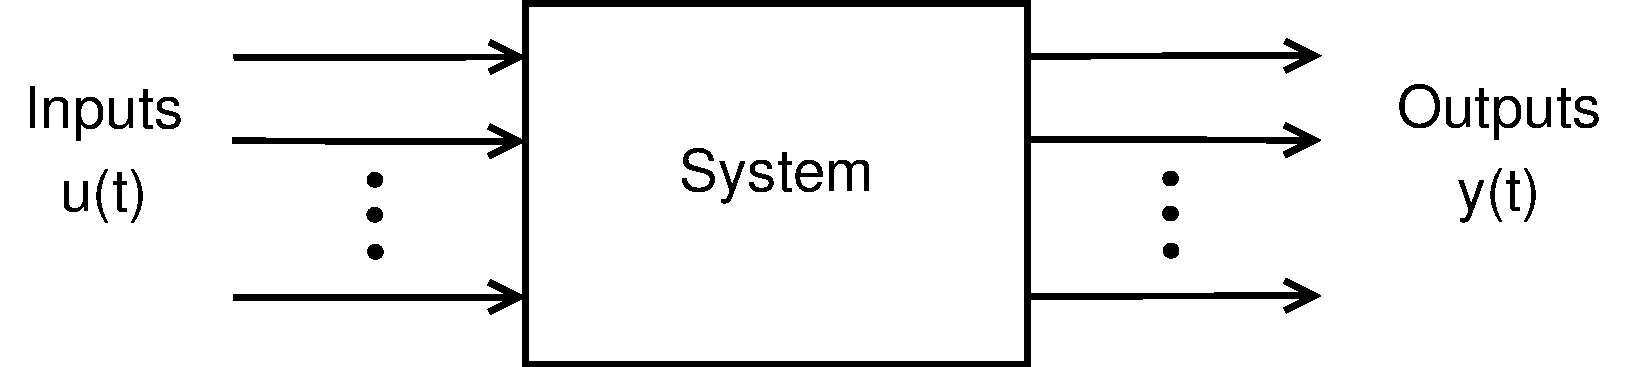
\includegraphics[width=.9\linewidth]{systems_theory}
	\end{figure}
	\bigskip
\end{frame}

\begin{frame}
	\frametitle{Systems theory}
	Next to inputs and outputs, states (denoted by \textbf x(t)) are a third type of variable used to describe a system. They represent the internal state of the system at a given time.\\
	\begin{center}
		$\dot{x}(t) = f(x(t),u(t))$\\
		$y(t) = g(x(t),u(t))$\\
	\end{center}
	The order of a system is the number of state-variables (i.e. the size of the vector \textbf x).\\
	\bigskip
\end{frame}

\begin{frame}
	\frametitle{Dynamical system}
	A dynamical system is a constantly changing system that connects outputs and inputs.\\The word dynamical refers to the fact that its current output depends on past input, contrary to static systems where the current output only depends on current input. This means that in a dynamical system the output changes with time if the system is not in a state of equilibrium.\\
	\medskip
	Everything is a dynamical system.\\
	Example:\\
	\begin{figure}
		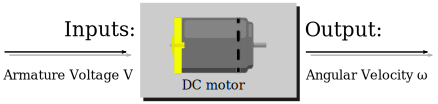
\includegraphics[width=0.7\linewidth]{dc_motor}
	\end{figure}
\end{frame}

\section{Real life examples} 

\begin{frame}
	\frametitle{Millenium Bridge}
	Resonance on the Millenium Bridge in London due to the rithm of walking people.
	\begin{figure}
		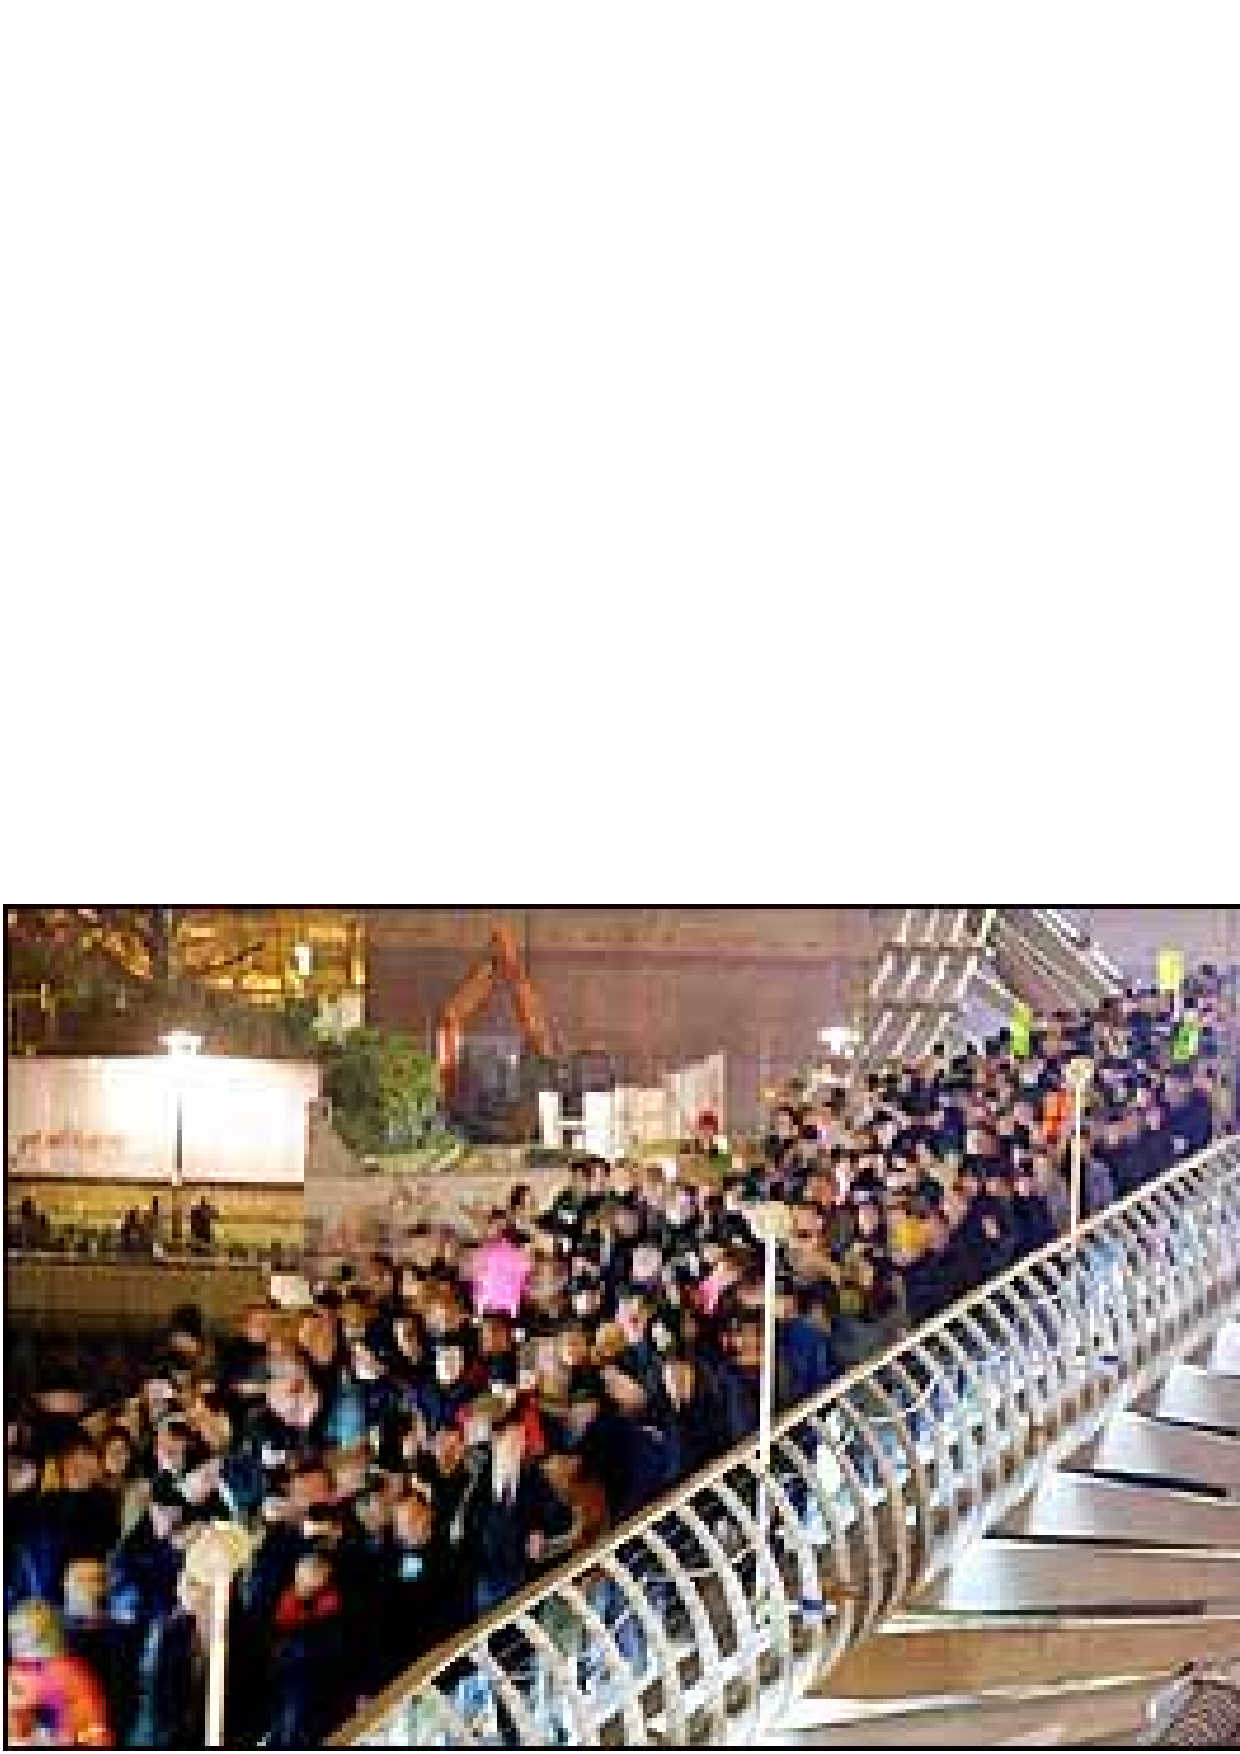
\includegraphics[scale=0.3]{millenium_bridge}
	\end{figure}
	\url{https://www.youtube.com/watch?v=eAXVa__XWZ8}
\end{frame}

\begin{frame}
	\frametitle{Neuronal acitvity}
	Real-time visualization of neuronal activity in the zebrafish brain
	\begin{figure}
		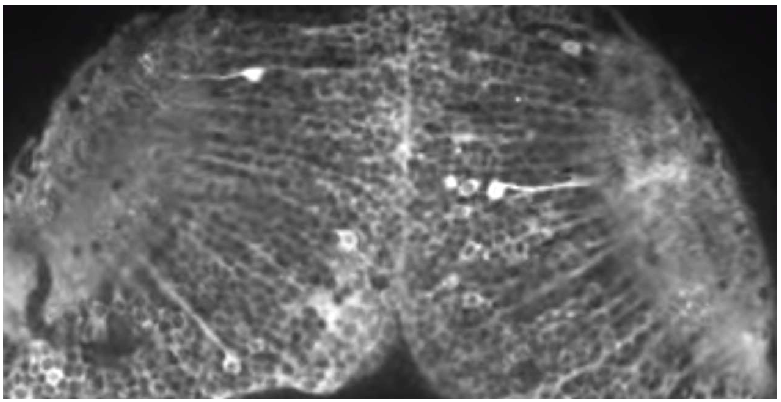
\includegraphics[scale=0.7]{neuronal_activity}
	\end{figure}
	\url{https://youtu.be/_rGEkYfQVwY}
\end{frame}

\begin{frame}
	\frametitle{Drumstick hitting a cymbal}
	Drumstick hitting a cymbal at 1000 frames/sec
	\begin{figure}
		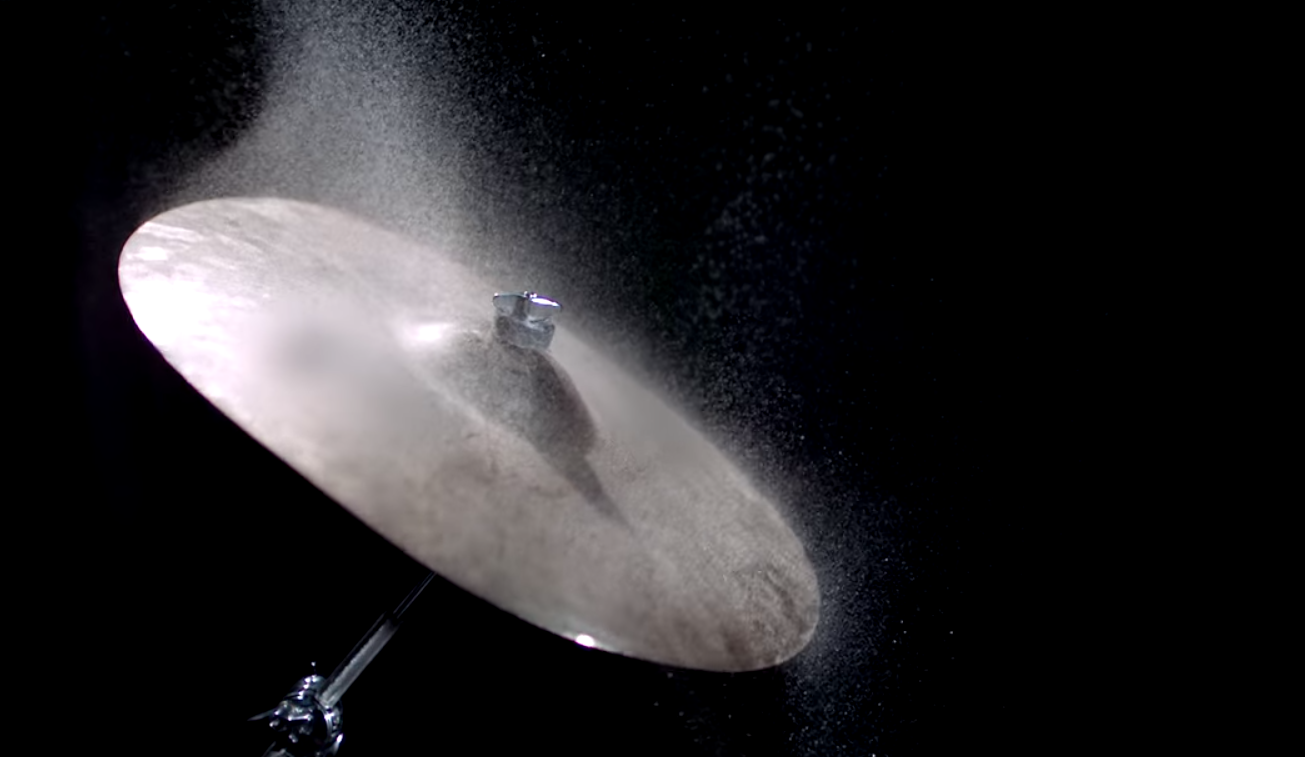
\includegraphics[scale=.6]{cymbal}
	\end{figure}
	\url{https://youtu.be/kpoanOlb3-w}
\end{frame}

\begin{frame}
	\frametitle{Pilot making a risky maneuvre}
	Experienced pilot making a risky maneuvre
	\begin{figure}
		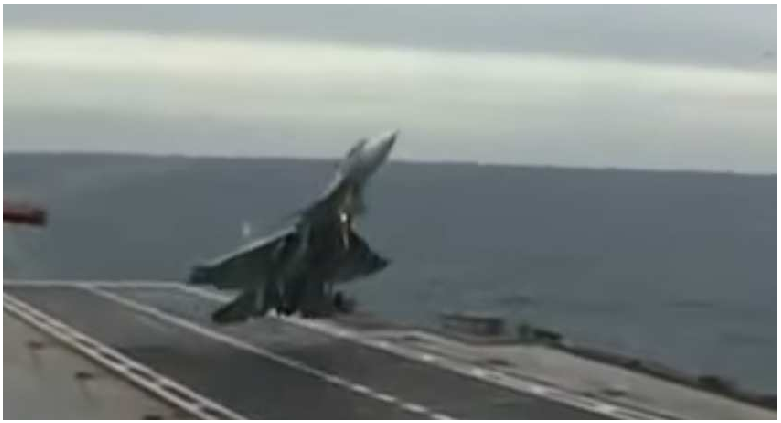
\includegraphics[scale=0.7]{risky_maneuvre}
	\end{figure}
	\url{https://youtu.be/gGnyWgXnZ6g}
\end{frame}

\begin{frame}
	\frametitle{Synchronized metronomes}
	Synchronized metronomes
	\begin{figure}
		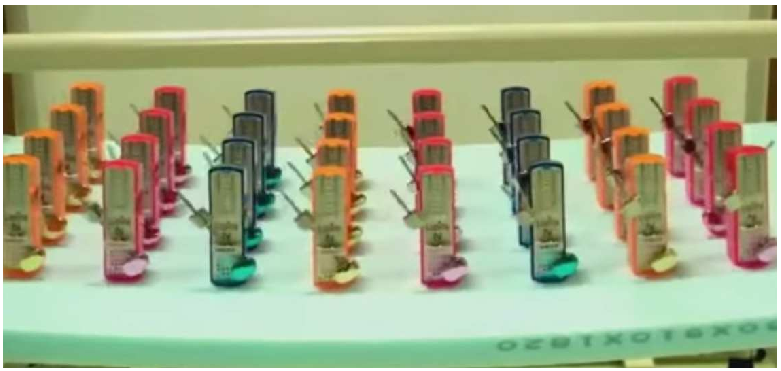
\includegraphics[scale=0.8]{synchronized_metronomes}
	\end{figure}
	\url{https://www.youtube.com/watch?v=5v5eBf2KwF8}
\end{frame}

\section{Control theory}

\begin{frame}
	\frametitle{Control theory}
	Control theory deals with the behavior of dynamical systems and how their behavior is modified by feedback.\\
	The output is compared to the reference signal and this \textit{'error'} is used by the controller to adjust the system. 
	\medskip
	\begin{figure}
		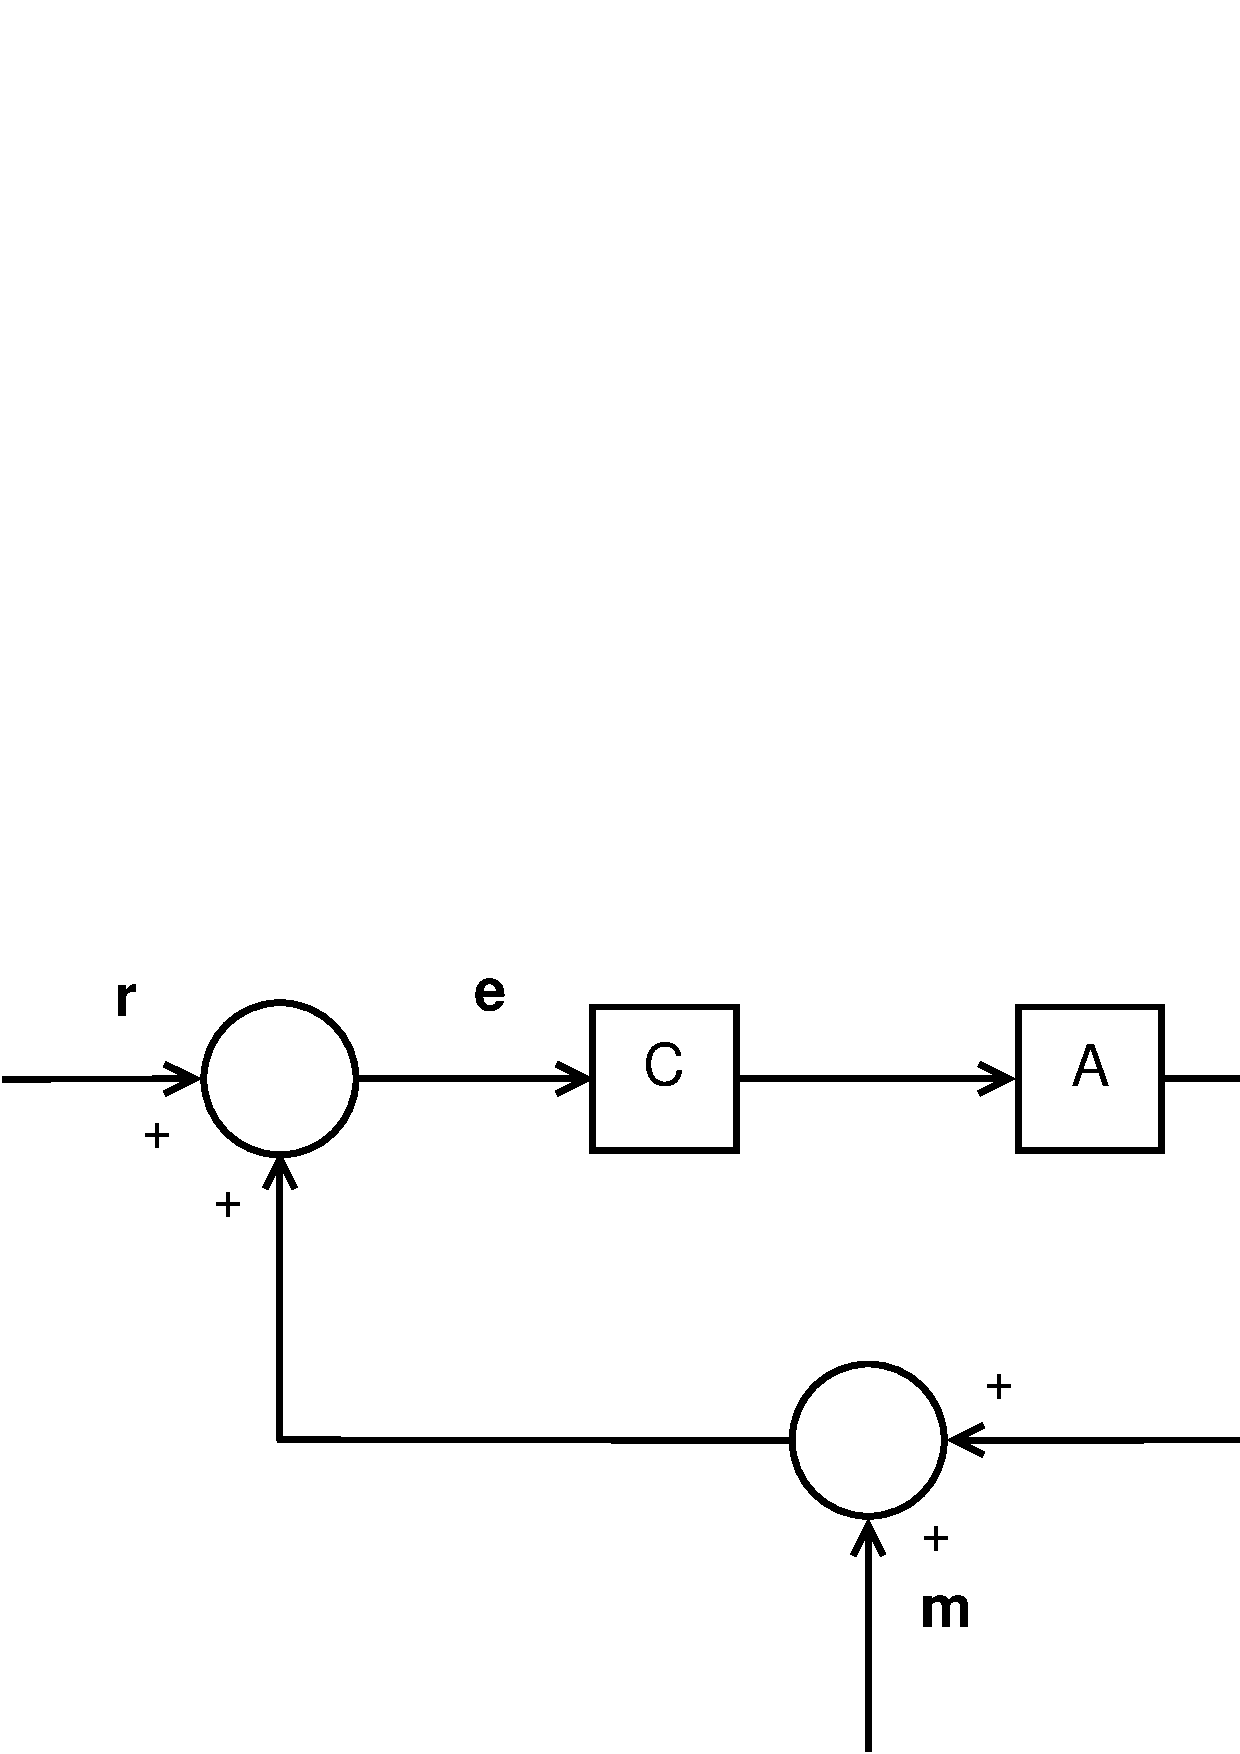
\includegraphics[width=1\linewidth]{full_system1}
	\end{figure}
\end{frame}

\begin{frame}
	\frametitle{Control theory}
	\begin{figure}
		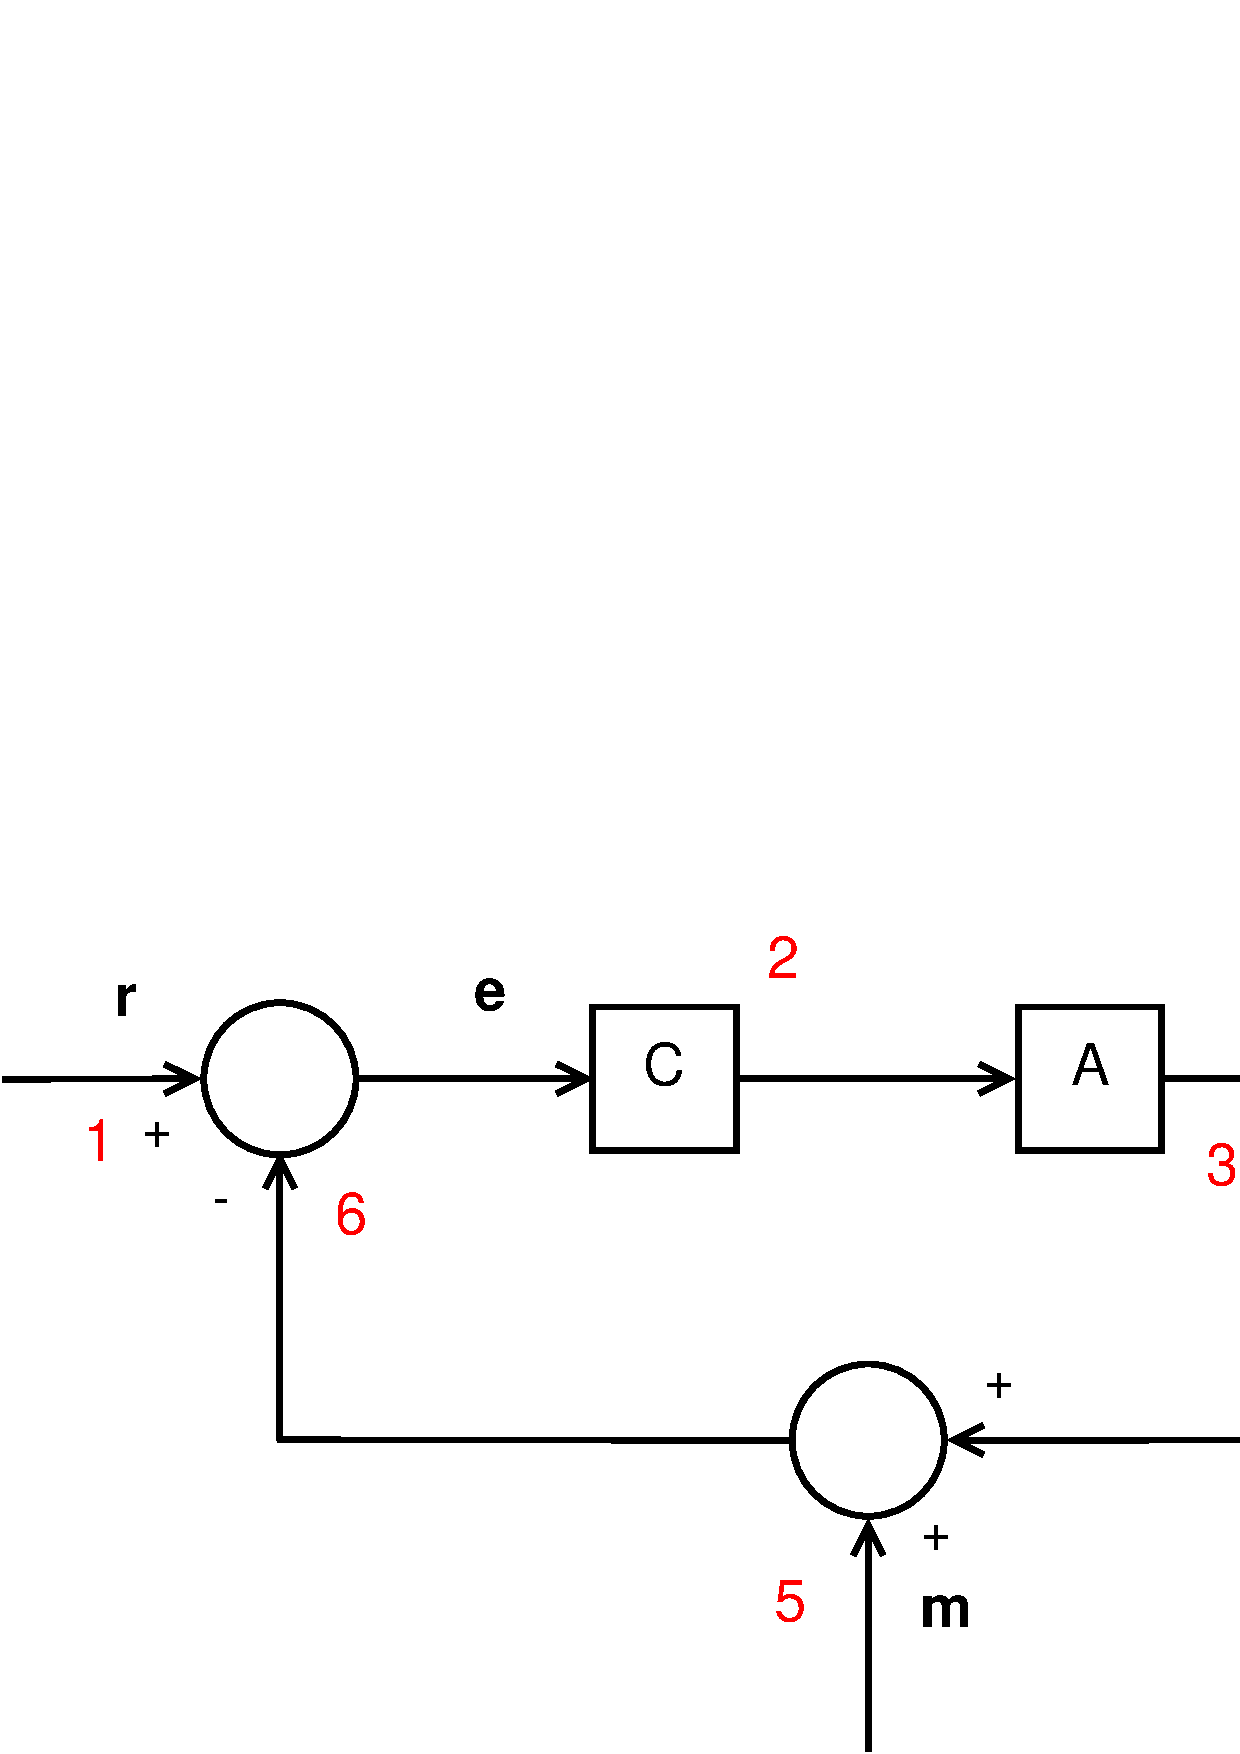
\includegraphics[width=.8\linewidth]{full_system2}
	\end{figure}
	\vspace{-2ex}
	1. Reference signals: the desired output signals\\
	2. Controller\\
	3. Actuators\\
	4. Noise\\
	5. Measurement noise\\
	6. Negative feedback
\end{frame}

\begin{frame}
	\frametitle{Example}
	\vspace{-6ex}
	Speed control system\\
	\bigskip
	\bigskip
	\begin{figure}
		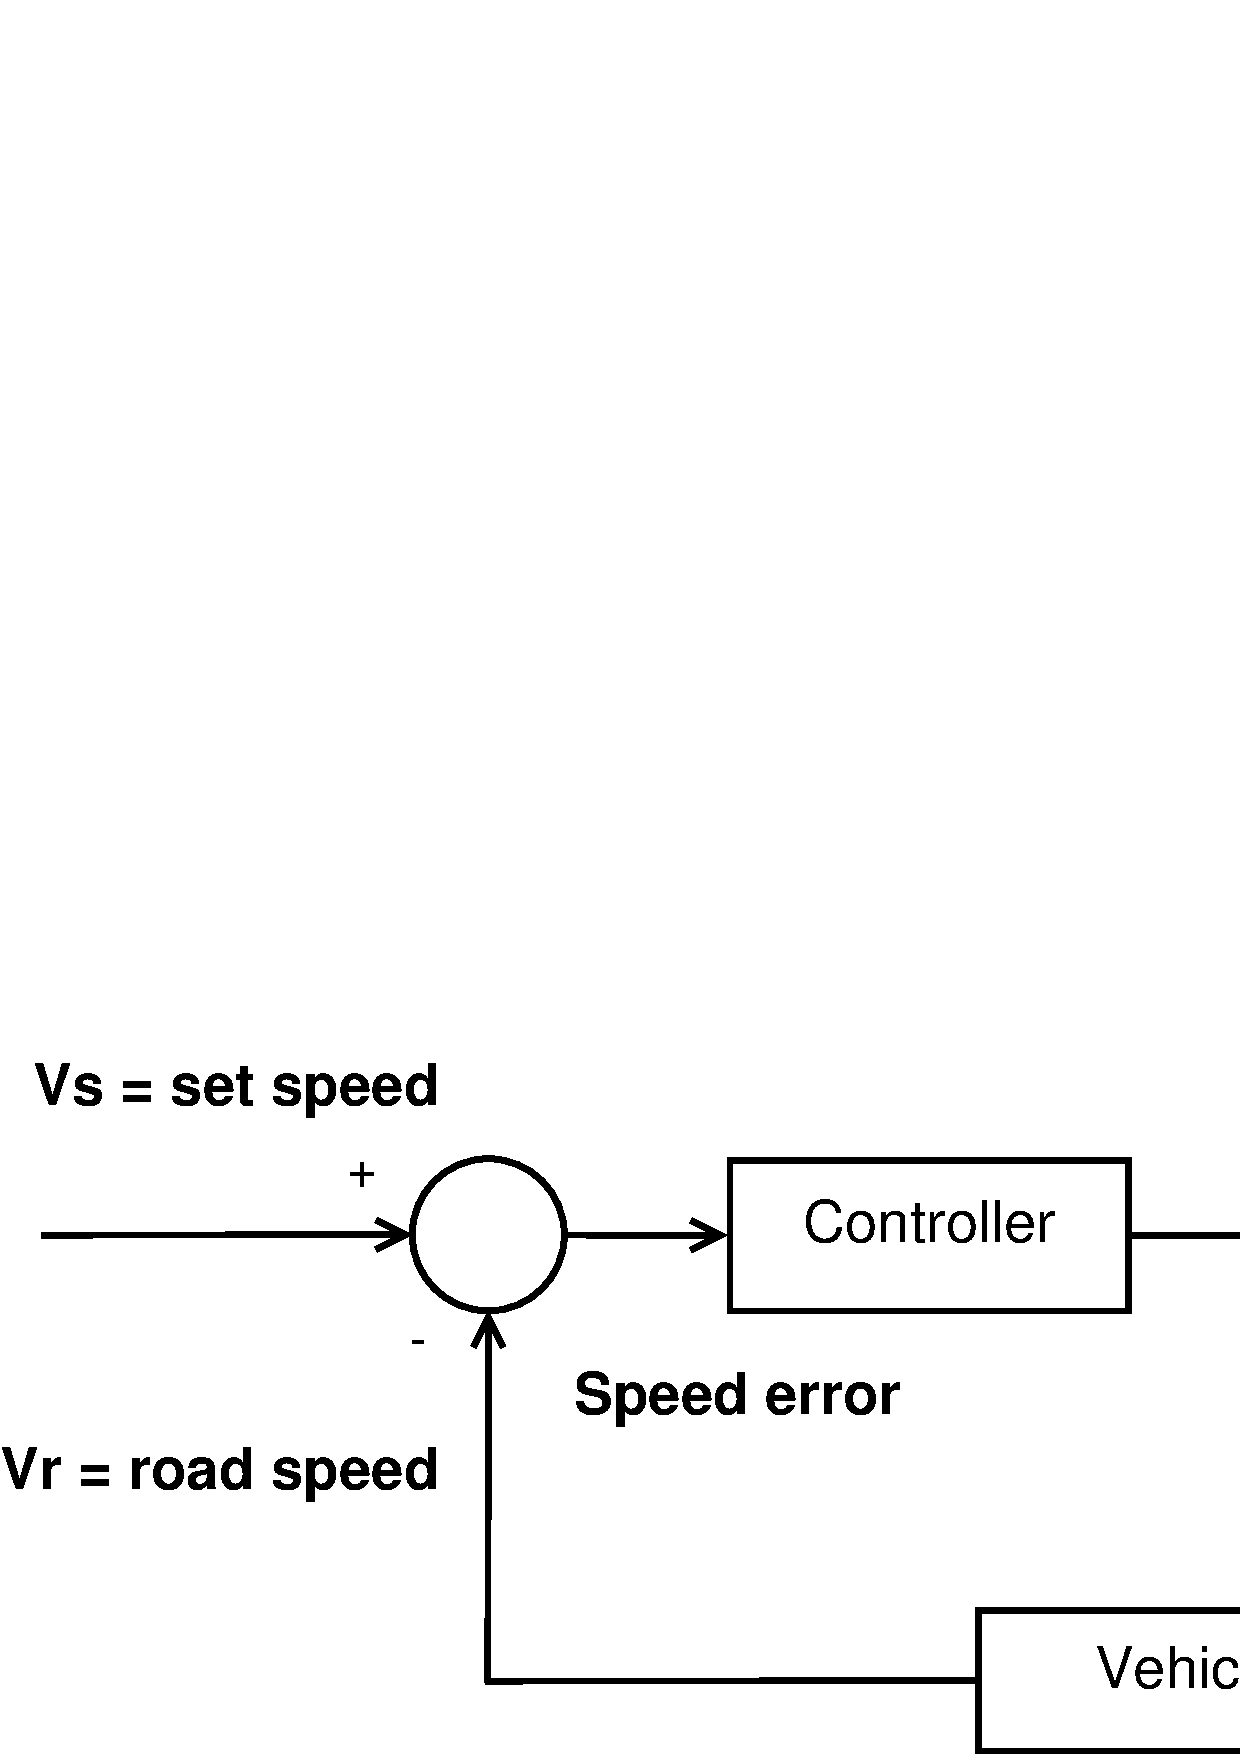
\includegraphics[width=1\linewidth]{speed_control_system}
	\end{figure}
\end{frame}


\begin{frame}
	\frametitle{Example}
	\vspace{-3ex}
	Temperature control system\\
	\bigskip
	\begin{figure}
		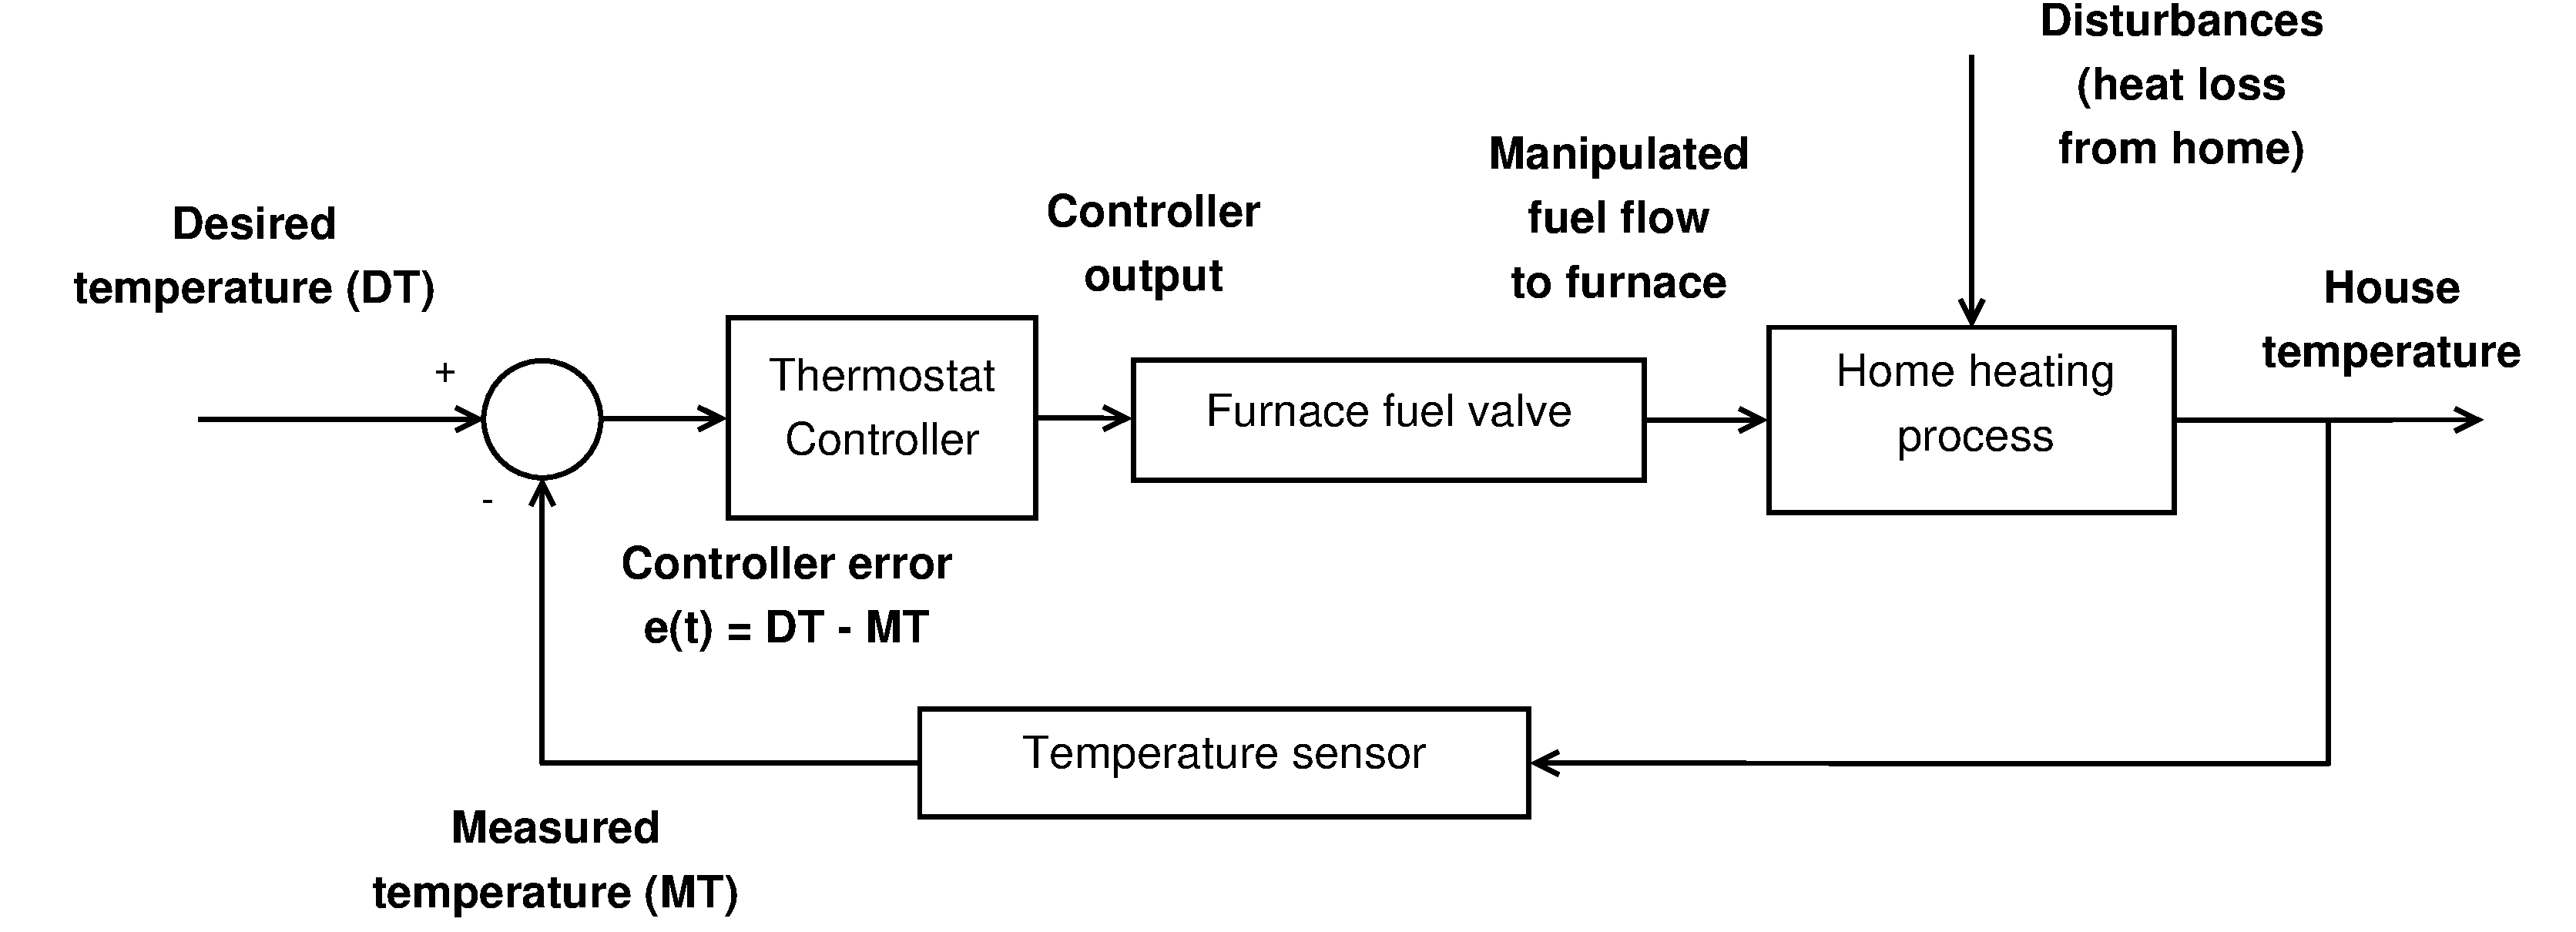
\includegraphics[width=1\linewidth]{temp_control_system}
	\end{figure}
\end{frame}


\begin{frame}
	\frametitle{Automation}
	\begin{figure}
		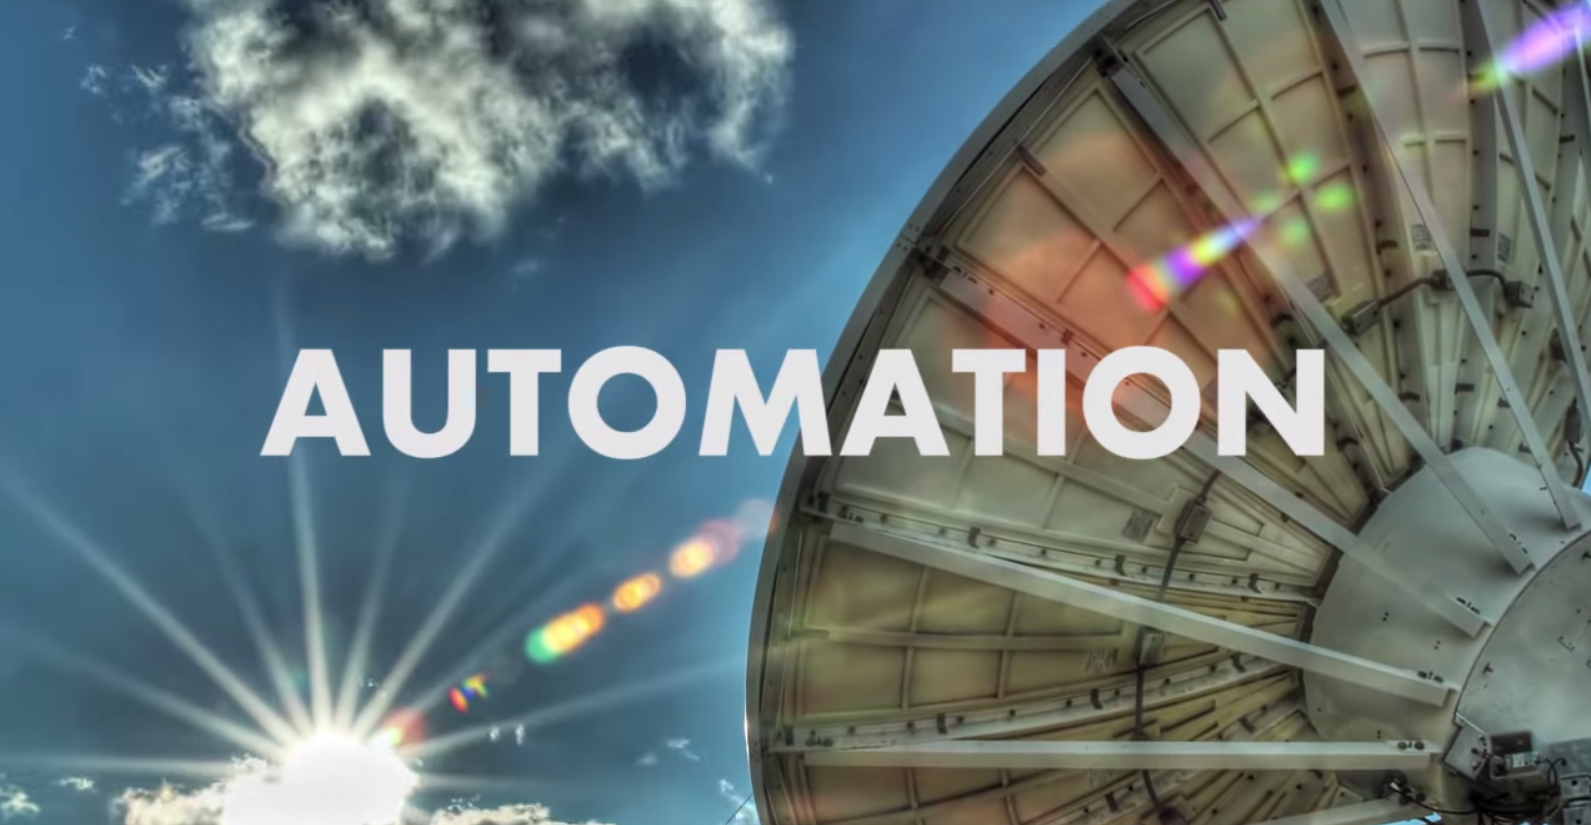
\includegraphics[width=1\linewidth]{automation}
	\end{figure}
	\url{https://youtu.be/XJLMW6l303g}
\end{frame}

\section{Open-loop vs. closed-loop systems} 

\begin{frame}
	\frametitle{Open loop}
	\vspace{-4ex}
	In an open loop system, the output is not fed back into the controller. Therefore, the controller cannot \textit{'see'} the effect of its actions. \\
	This way it is hard to get the desired output.\\
	\bigskip
	\begin{figure}
		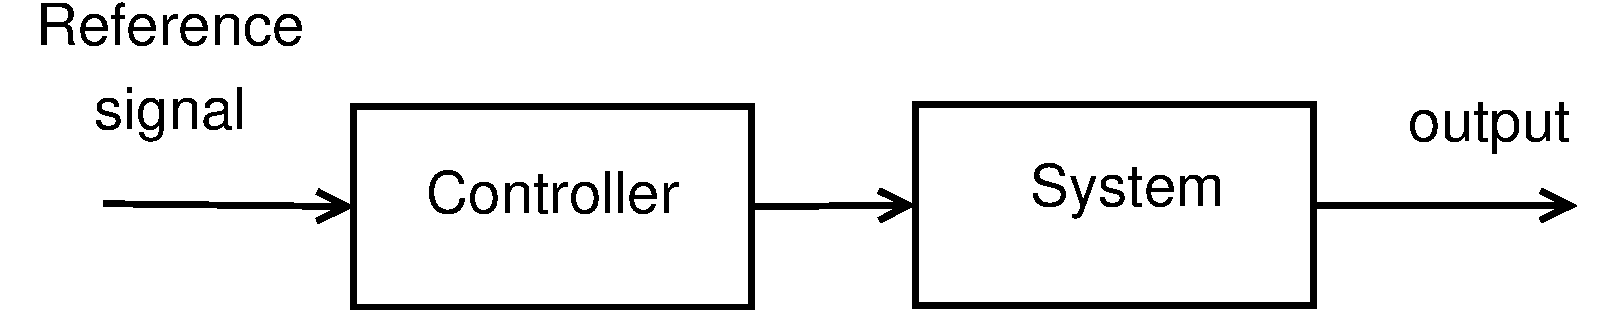
\includegraphics[width=1\linewidth]{open_loop}
	\end{figure}
\end{frame}

\begin{frame}
	\frametitle{Open loop}
	\begin{columns}[c]
		
		\column{.6\textwidth}
		Take for example the following system:\\
		\begin{itemize}
			\item You are pouring a glass of water, but you \textbf{cannot look at the glass}.
			\item The desired output is a full glass of water within a reasonable time.
			\item The input can have two values: on or off (assume a quite primitive tap).
			\item It will not be easy to do this successfully.
		\end{itemize}
		
		\column{.4\textwidth}
		\begin{figure}
			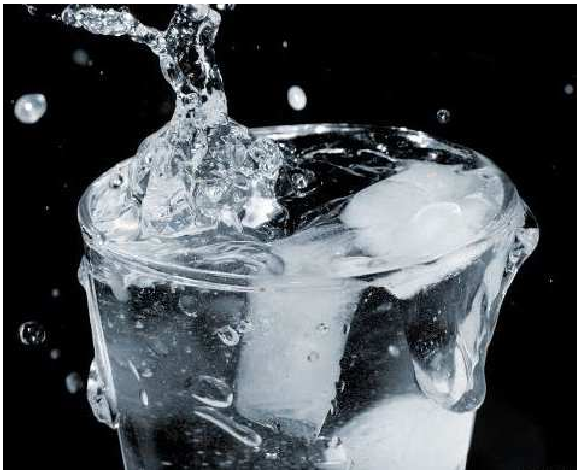
\includegraphics[width=1\linewidth]{glass}
		\end{figure}
		
	\end{columns}
	\bigskip
	The solution is evident: look at the glass while pouring!
\end{frame}

\begin{frame}
	\frametitle{Closed loop (feedback)}
	In a closed loop system, the error signal, which is the difference between the input signal and the output, is fed to the controller so as to reduce the error and bring the output to the desired value. 
	\medskip
	\begin{figure}
		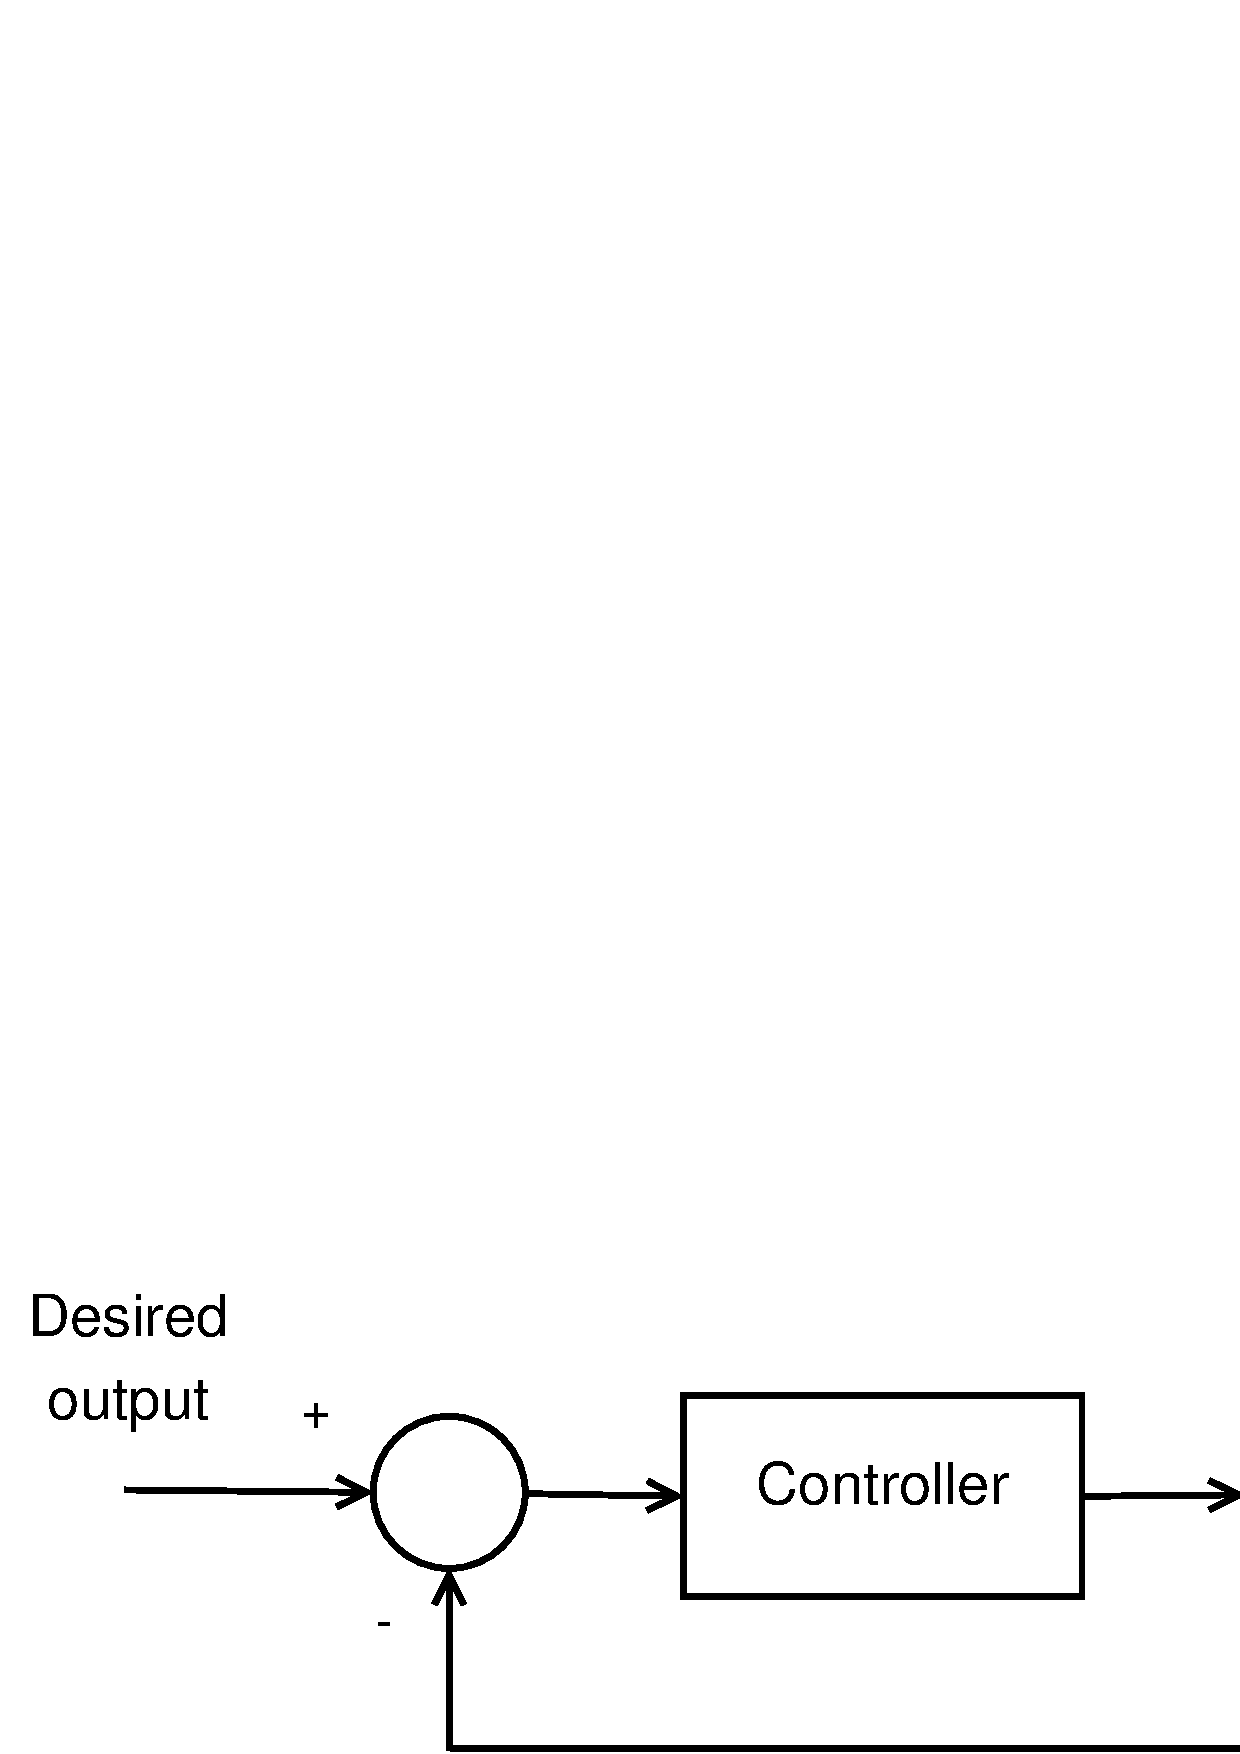
\includegraphics[width=1\linewidth]{closed_loop}
	\end{figure}
	\medskip
	There are two types of feedback systems. The output can either be added to the reference input (positive feedback) or substracted from it (negative feedback).
\end{frame}

\begin{frame}
	\frametitle{Guitar feedback}
	\begin{figure}
		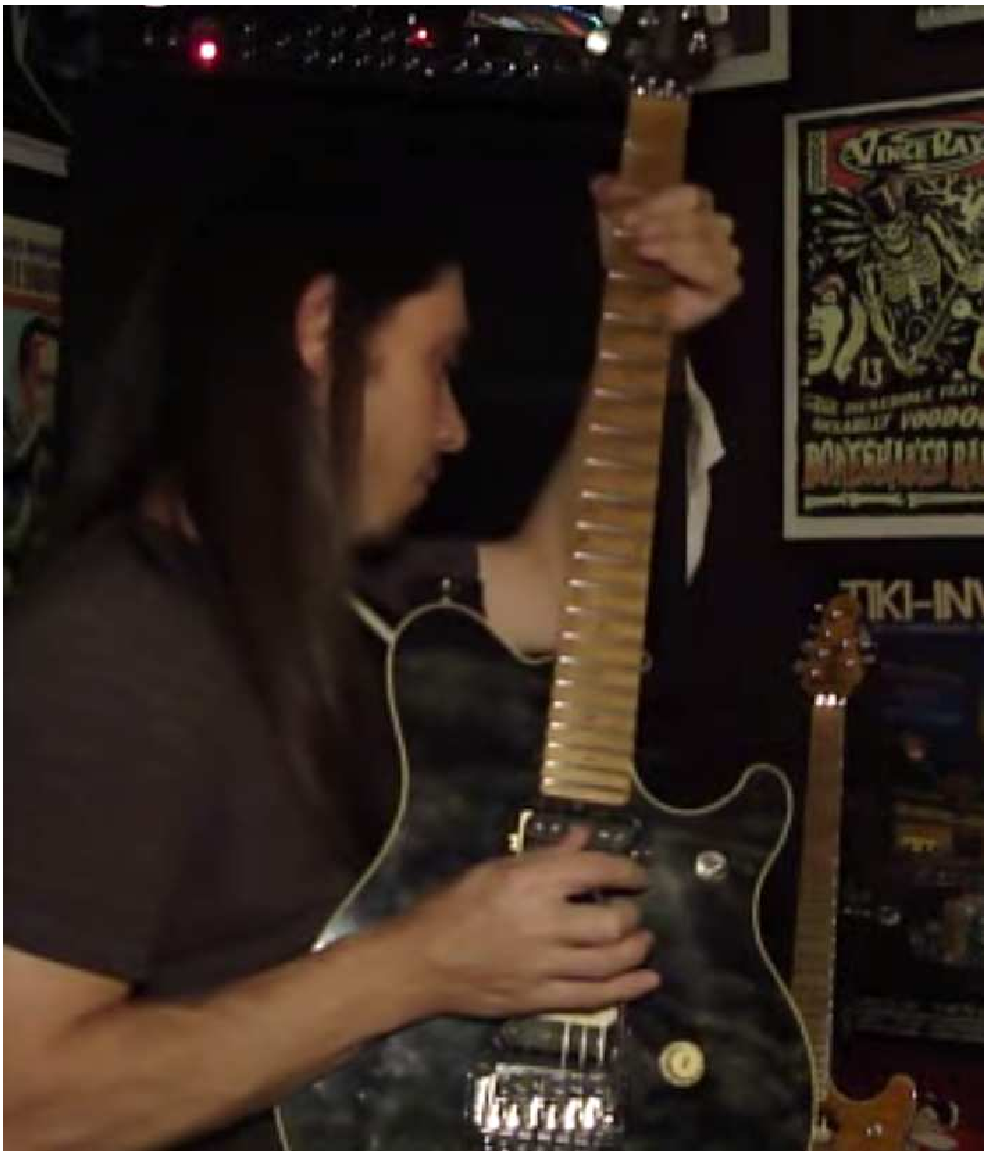
\includegraphics[width=.4\linewidth]{guitar}
	\end{figure}
	\url{https://youtu.be/luURyH9fzhk}
\end{frame}

\begin{frame}
	\frametitle{What if there was no feedback?}
	\begin{figure}
		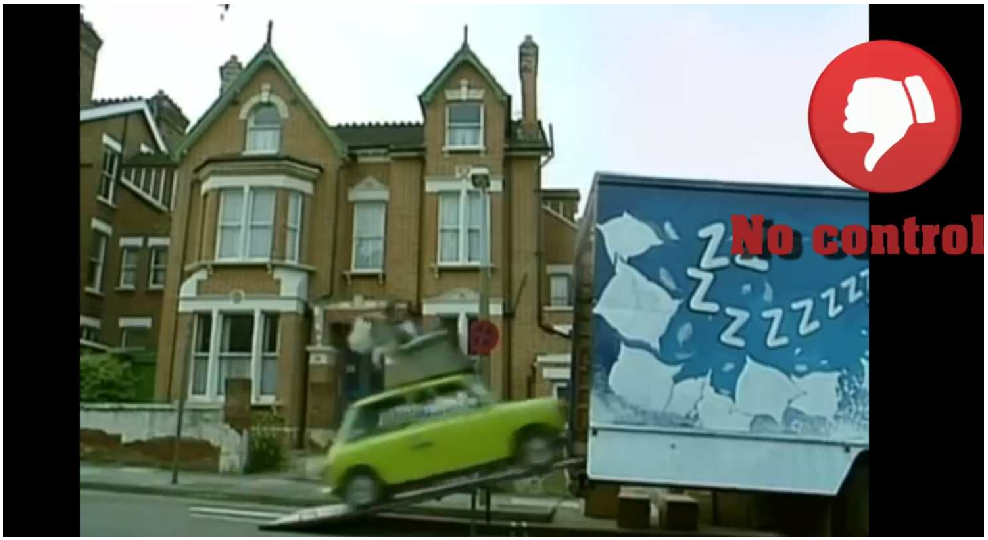
\includegraphics[width=.9\linewidth]{no_feedback}
	\end{figure}
	\url{https://youtu.be/C221sI1W9Gk}
\end{frame}

\begin{frame}
	\frametitle{Feedback loops in biology}
	\begin{figure}
		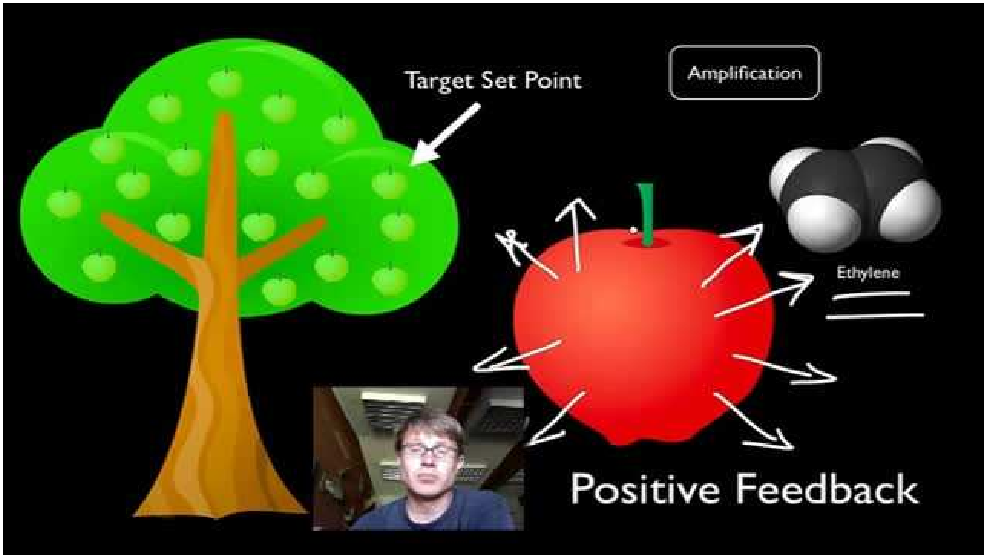
\includegraphics[width=.9\linewidth]{feedback_biology}
	\end{figure}
	\url{https://www.youtube.com/watch?v=CLv3SkF_Eag}
\end{frame}

\section{Automatic control} 

\begin{frame}
	\frametitle{Dance of the Flying Machines}
	\begin{figure}
		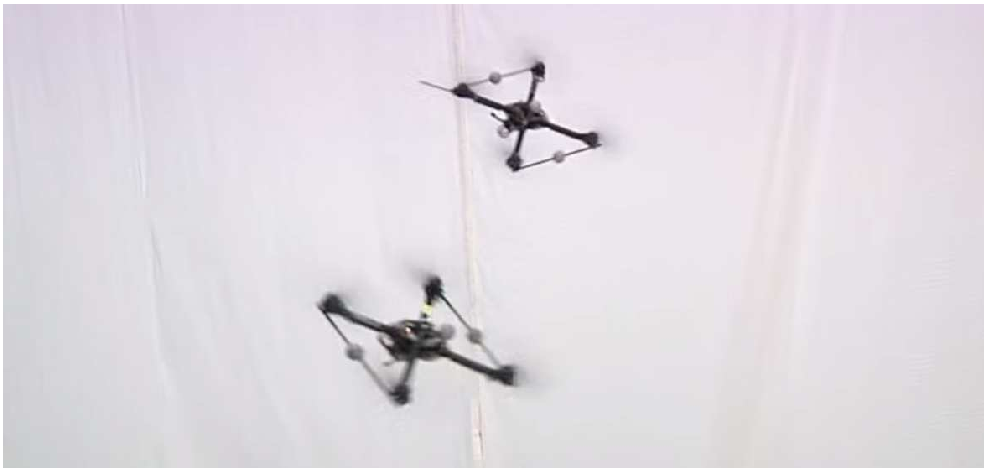
\includegraphics[scale=.6]{flying_machines}
	\end{figure}
	\url{https://youtu.be/NRL_1ozDQCA}
\end{frame}

\begin{frame}
	\frametitle{Automated driving with precision at the physical limits}
	\begin{figure}
		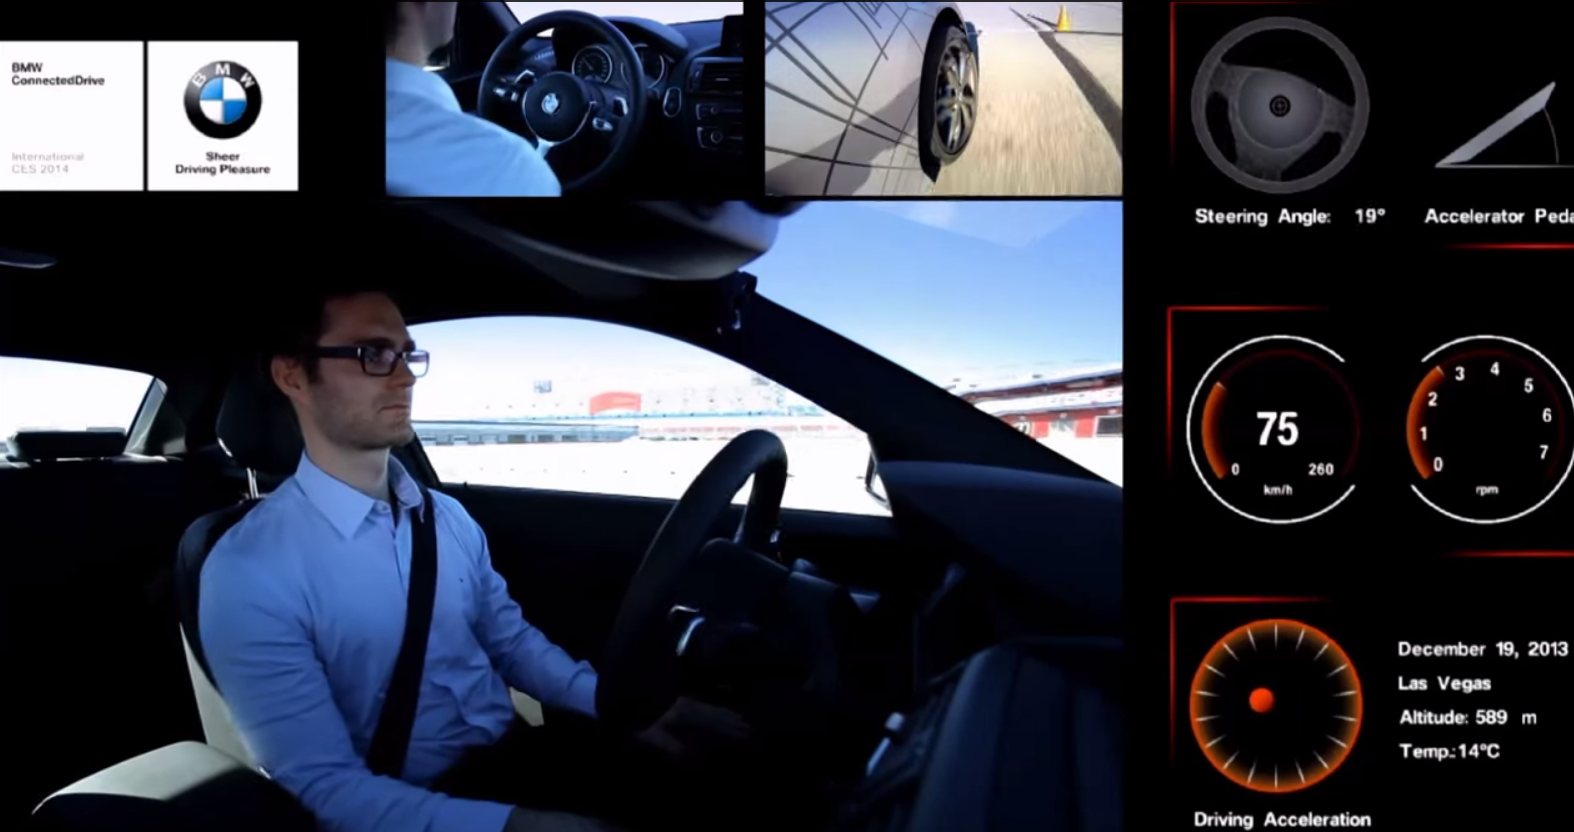
\includegraphics[scale=.6]{autonomous_car}
	\end{figure}
	\url{https://youtu.be/1FVglbJZ_tg}
\end{frame}

\begin{frame}
	\frametitle{The Cubli: a cube that can jump, balance and 'walk'}
	\begin{figure}
		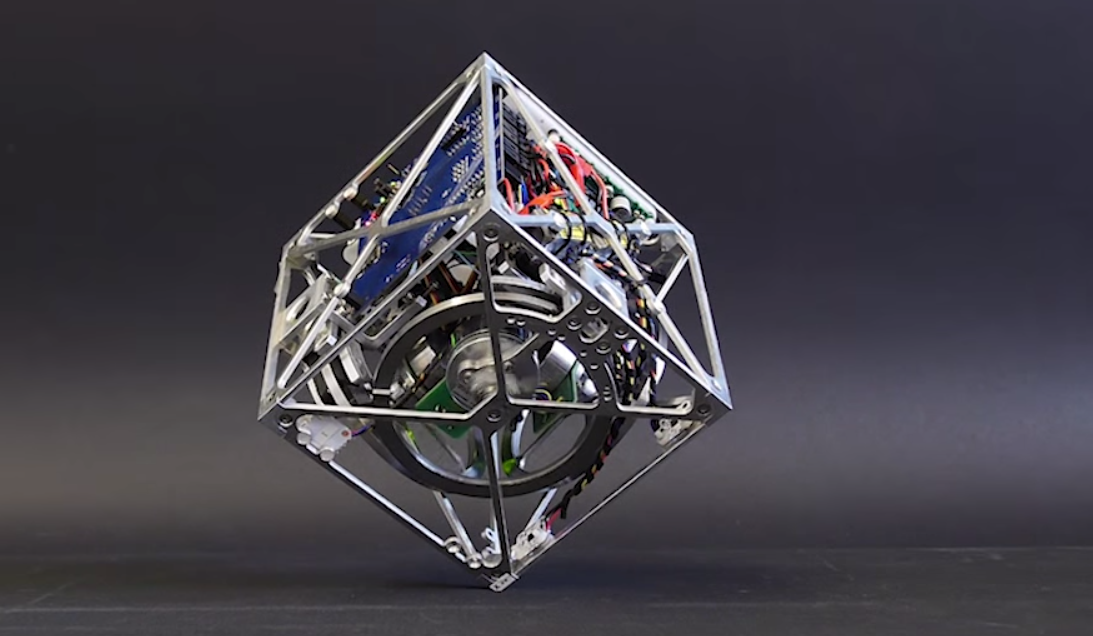
\includegraphics[scale=.55]{cubli}
	\end{figure}
	\url{https://youtu.be/n_6p-1J551Y}
\end{frame}

\begin{frame}
	\frametitle{Magnetic manipulator Magman and Matlab}
	\begin{figure}
		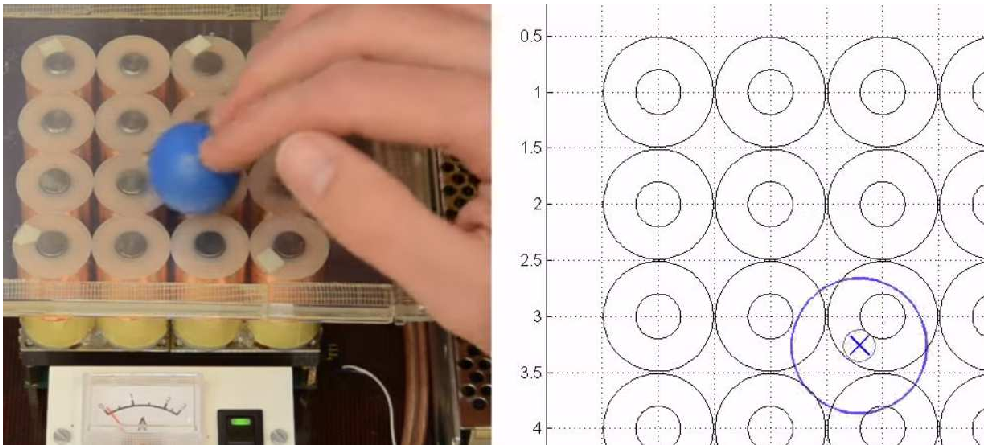
\includegraphics[scale=.65]{magnetic_manipulator}
	\end{figure}
	\url{https://youtu.be/AhS_2gU1qW0}
\end{frame}

\begin{frame}
	\frametitle{Badminton robot}
	\begin{figure}
		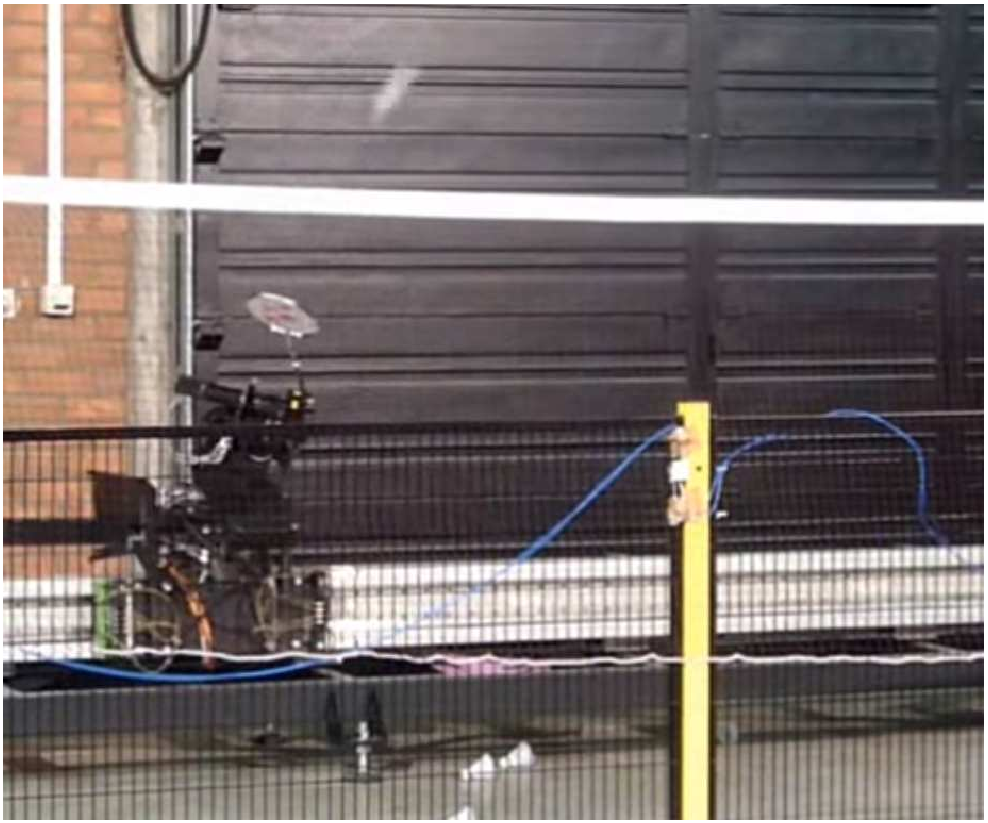
\includegraphics[scale=.4]{badminton_robot}
	\end{figure}
	\url{https://youtu.be/LSax71cn6A4}
\end{frame}

\begin{frame}
	\frametitle{Raffaello D'Andrea: The astounding athletic power of quadcopters}
	\begin{figure}
		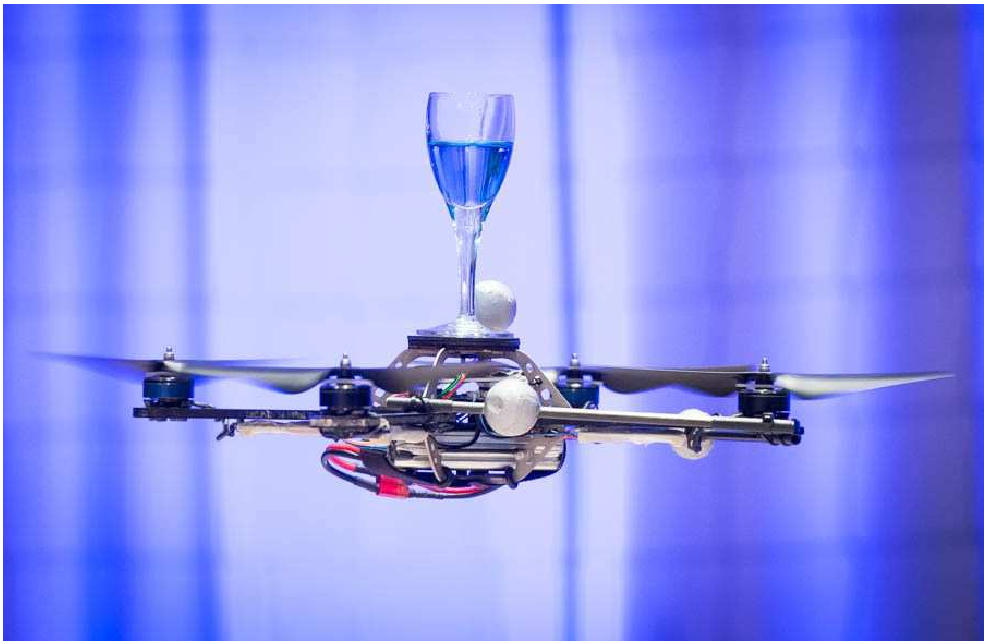
\includegraphics[scale=.4]{quadcopter}
	\end{figure}
	\url{https://www.youtube.com/watch?v=w2itwFJCgFQ}
\end{frame}